\chapter{Global Basis Time of Maximum and c}
\label{chap:fixing_t_c}

\section{Globally shared time of maximum and c}

Given the empirical results which confirm the efficiency and efficacy of the model with a shared value of $t_{max}$, the chapter wants to investigate the goodness of the model when commonly calibrating $t_{max}$ together with $c$, relying on the implemented framework which allows to reach the goal without substantial modifications. 
The further step with respect to the previous one is more fragile, because:

\begin{enumerate}
    \item it has not a financial foundation, indeed the input form has been changed because the parameters, $c$ included, can be interpreted from a physical but not financial point of view;
    \item the interest rate curve, and its basis too, needs at least 3 parameter for describing its 3 principal moments: short, medium and long term. Therefore, this modelling choice hopes to describe them with 2 unconstrained variables and 2 constrained ones.
\end{enumerate}

On the other hand, the model would acquire the flexibility to move from absolute and relative basis.
Only empirical results can justify this choice.
 
\subsection{Empirical results}

The problem can be written as:

\begin{equation*}
\begin{aligned}
& \underset{t_{max},c}{min}
& & \sqrt{\sum_{i=1}^{n}(\epsilon_{i}(a_{i},c,d_{i},t_{max}))^{2}w_{i}}\,, \\
\end{aligned}
\end{equation*}

where:

\begin{equation*}
\begin{aligned}
& \underset{a,d}{min}
& & \epsilon_{i}(a_{i},c,d_{i},t_{max})=\sqrt{\sum_{j=1}^{m_{i}}(p_{j}-r_{j}(a_{i},c,d_{i},t_{max}))^{2}w_{j}}\,. \\
\end{aligned}
\end{equation*} 

Considering both the global error described by \eqref{eq:global_error} which takes a value of 2.13 (sum of root mean square errors below reported) and the correction factors distribution the results are excellent:

\begin{figure}[H]
\centering
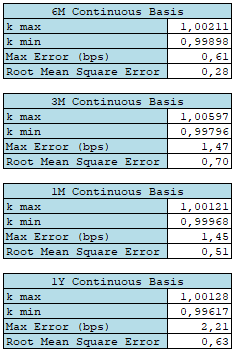
\includegraphics[scale=1]{k_no_inc_t_c}
\caption{Correction factors k from not incremental calibration with global $t_{max}$ and c}
\label{fig:k_no_inc_t_c}
\end{figure}

Range of $k$ values is closed to 1 that is the best value because indicates that no corrections are needed.
Moreover, the statistics follow:

\begin{figure}[H]
\centering
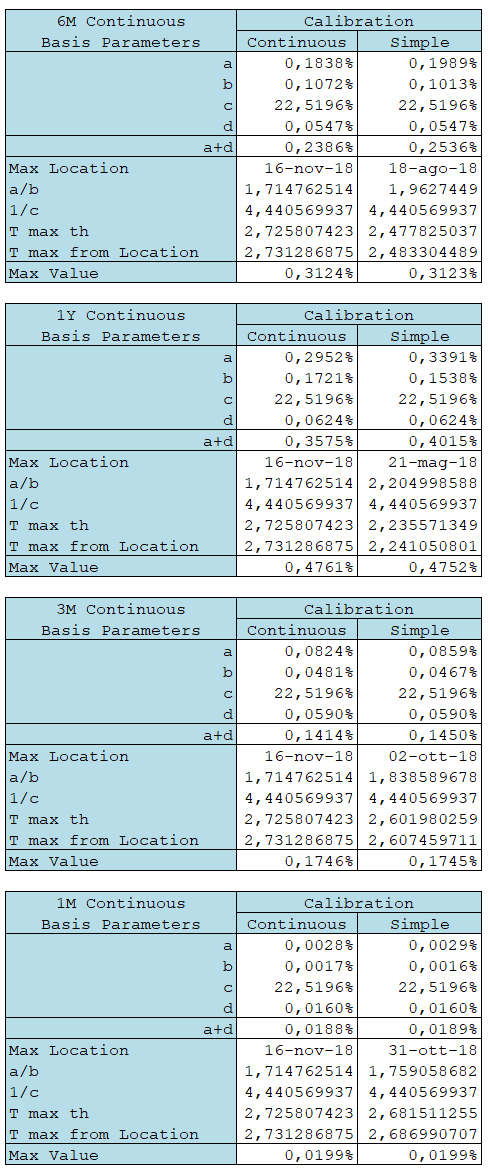
\includegraphics[scale=1]{acdt_Parameters_t_c}
\caption{Parameters from not incremental calibration with global $t_{max}$ and c}
\label{fig:acdt_Parameters_t_c}
\end{figure}

The only problem which arises it is the same as before with the legacy curve for 3M and 12M tenor and it should be faced in the same way, therefore no further explanations are required.

Anyway, the global $t_{max}$ calibration matter about 1M shape and $d$ convergence seems to find another confirm of the initial intuition, once removed the noise and fixed $t_{max}$ the constrained on $c$ allows to retrieve what is theoretically expected:

\begin{figure}[H]
\centering
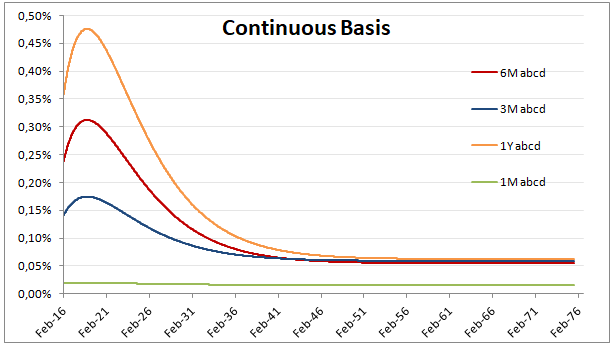
\includegraphics[scale=0.85]{graph_basis_comparison_no_inc_t_c}
\caption{Absolute basis from not incremental calibration with global $t_{max}$ and c}
\label{fig:graph_basis_comparison_no_inc_t_c}
\end{figure}

Once again, although remembering that the index which points to an acdt basis should be corrected with the $k$ factors in order to perfectly reprice the provided market quotes, it is interesting to look at the repricing errors for each tenor:

\begin{figure}[H]
\centering
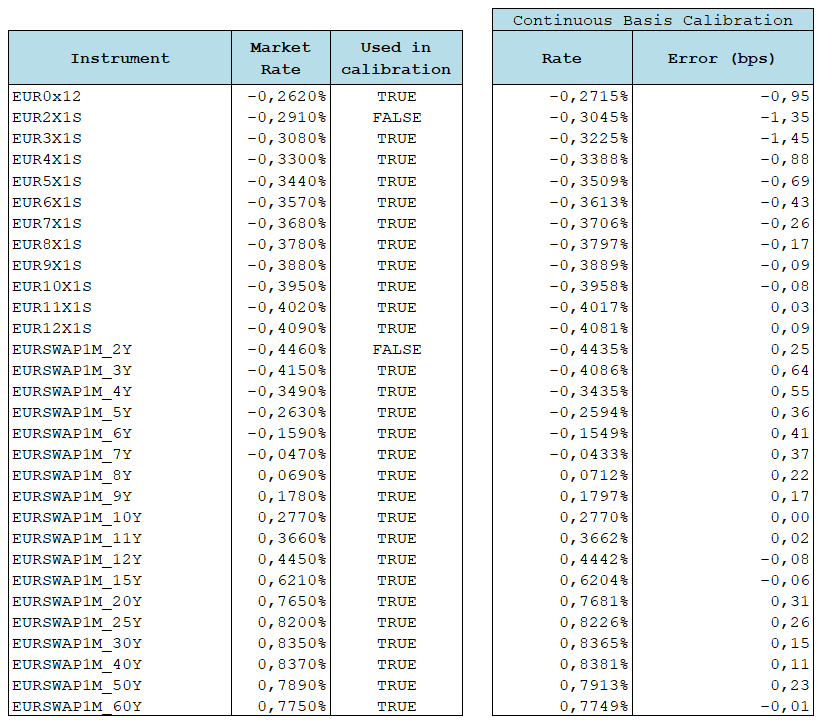
\includegraphics[scale=1]{1Merror_t_c}
\caption{1M instruments index repricing errors with global $t_{max}$ and c}
\label{fig:1Merror_t_c}
\end{figure}

\begin{figure}[H]
\centering
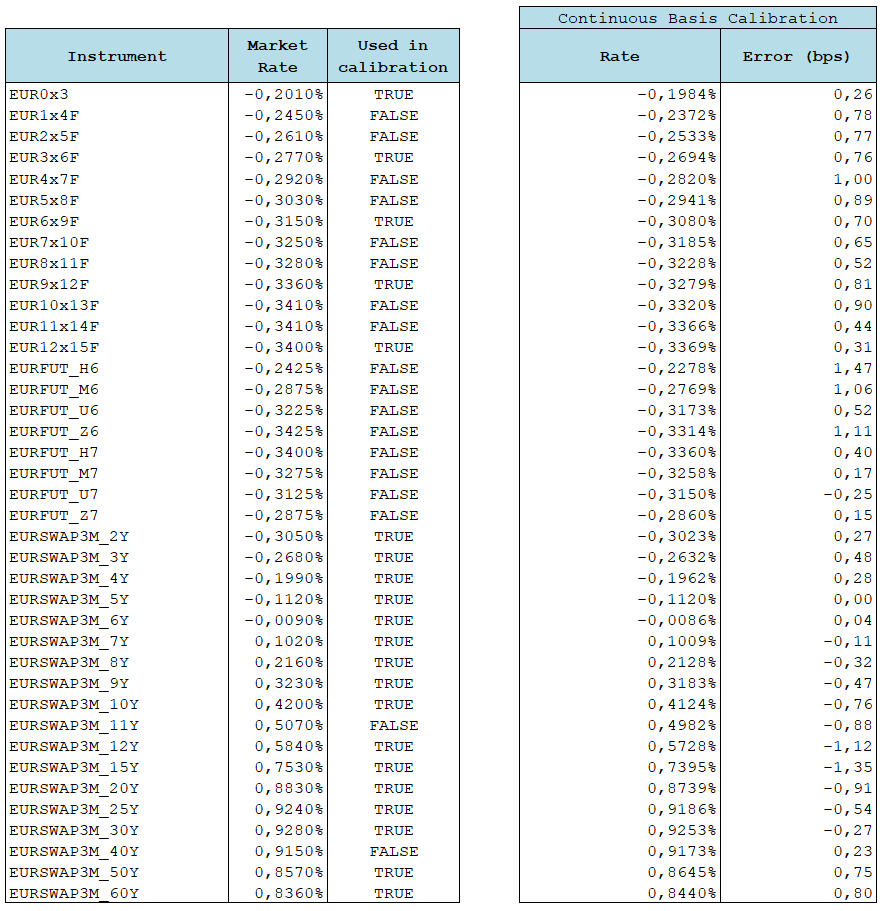
\includegraphics[scale=1]{3Merror_t_c}
\caption{3M instruments index repricing errors with global $t_{max}$ and c}
\label{fig:3Merror_t_c}
\end{figure}

\begin{figure}[H]
\centering
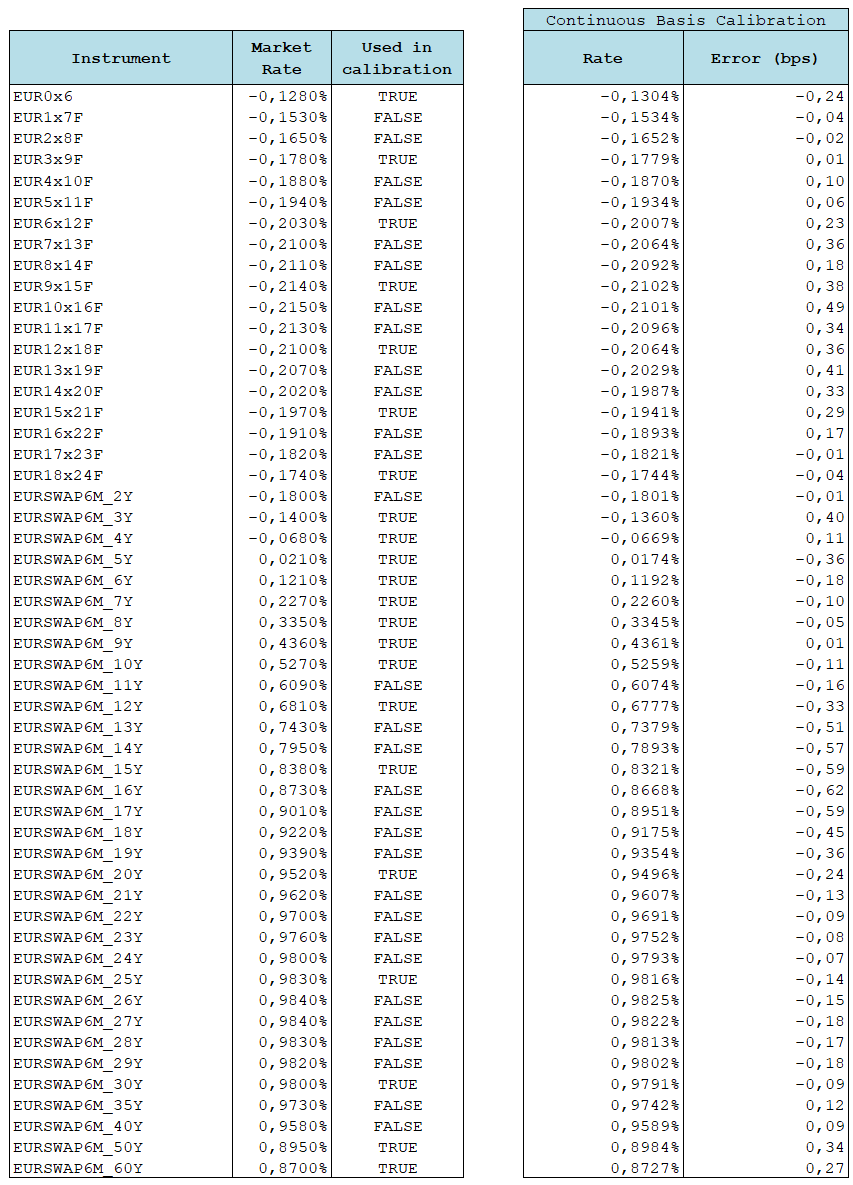
\includegraphics[scale=1]{6Merror_t_c}
\caption{6M instruments index repricing errors with global $t_{max}$ and c}
\label{fig:6Merror_t_c}
\end{figure}

\begin{figure}[H]
\centering
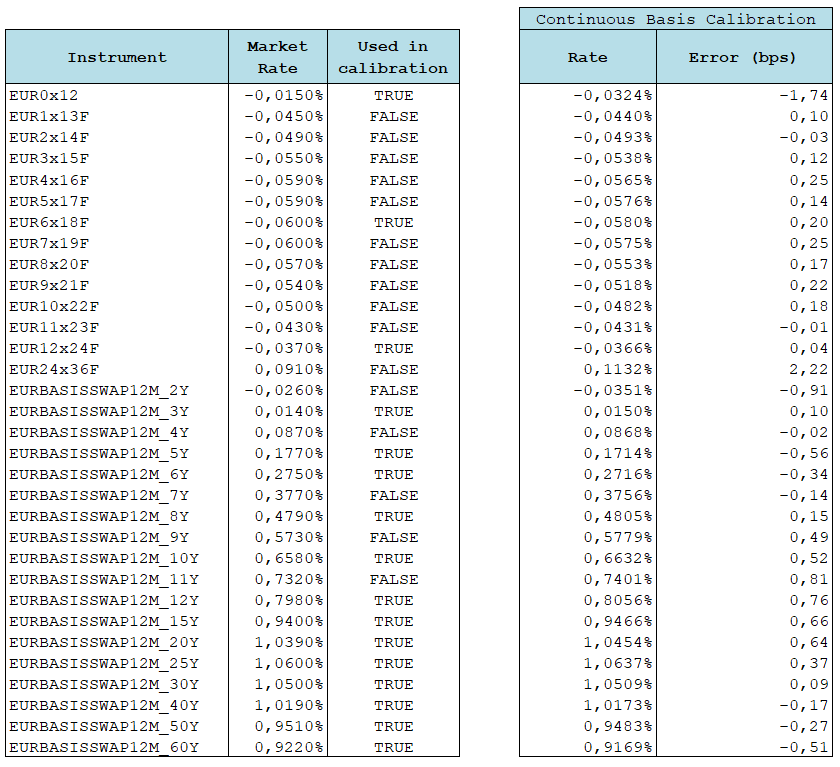
\includegraphics[scale=1]{12Merror_t_c}
\caption{12M instruments index repricing errors with global $t_{max}$ and c}
\label{fig:12Merror_t_c}
\end{figure}

Always assuming a market bid ask spread of 1 basis point all the models but 3M can be considered reliable for an effective employment in a trading desk.
The main findings from this empirical evaluation are:

\begin{itemize}
    \item goodness of fit which demonstrates the validity of the approach;
    \item possibility to shift to incremental basis.
\end{itemize}


\section{Basis shifting}


Certified that also with a fixed value of $c$ the model works, in the following theoretical results are studied together with testing the capabilities of repricing market quotes exploiting basis retrieved thanks to \eqref{eq:still_abcd}.

\subsection{Retrieving parameters}

After globally calibrated the model, where absolute basis have been built according to the abcd framework as \eqref{eq:forward as basis + on}, the relative basis can be retrieved thanks to \eqref{eq:still_abcd}.

In particular have been retrieved:

\begin{equation}
  s_{x,6M}=s_{x}-s_{6M}
\end{equation}

where: $x\in{(1M, 3M, 12M)}$ 

while for the 1M according to the incremental principle it has been additionally retrieved:

\begin{equation}
  s_{x,3M}=s_{x}-s_{3M}
\end{equation}

The parameters of $s_{x,y}$ have been retrieved exploiting \eqref{eq:x_y_parameters}.

If $x>y$:

\begin{equation*}
\begin{split}
a_{x,y}= a_{x} - a_{y};\\
b_{x,y}= b_{x} - b_{y} ;\\
d_{x,y}= d_{x} - d_{y} ;\\
\end{split}
\end{equation*}

otherwise:

\begin{equation*}
\begin{split}
a_{x,y}= a_{y} - a_{x};\\
b_{x,y}= b_{y} - b_{x} ;\\
d_{x,y}= d_{y} - d_{x} .\\
\end{split}
\end{equation*}

Given the basis, for each one has been made the repricing of the market quotes, modelling the considered instantaneous forward rate as:

\begin{equation}
  f_{x}=f_{ON} + s_{y} \pm s_{x,y}\,,
\end{equation}

where the sign of the relative basis depends on whether or not the considered $x$ tenor is greater or smaller than $y$.

Once explained the algorithm mechanism considerations are needed.

\subsection{Global basis time of maximum and c property}

Given the common absolute basis calibration of $t_{max}$ and $c$ for a pair of generic tenor $x$ and $y$, the following equations are valid:

\begin{equation}
    \frac{a_{x}}{b_{x}}=\frac{a_{y}}{b_{y}}\,,
    \label{eq:same_ratio_ab}
\end{equation}

\begin{equation*}
    t_{max}=\frac{1}{c}-\frac{a_{x}}{b_{x}}
\end{equation*}

and

\begin{equation*}
    t_{max}=\frac{1}{c}-\frac{a_{y}}{b_{y}}\,.
\end{equation*}

Looking at the $t_{max}$ functional form of their relative basis

\begin{equation*}
    t_{max}(x,y)=\frac{1}{c}-\frac{a_{x,y}}{b_{x,y}}\,,
\end{equation*}

in a verbose way:

\begin{equation*}
    t_{max}(x,y)=\frac{1}{c}-\frac{a_{x}-a_{y}}{b_{x}-b_{y}}\,.
\end{equation*}

Given that in order to obtain an abcd form of $s_{x,y}$ $c$ has been commonly calibrated, $t_{max}$ equals $t_{max}(x,y)$ if and only if:

\begin{equation}
    \frac{a_{x}}{b_{x}}=\frac{a_{x}-a_{y}}{b_{x}-b_{y}}\,.
    \label{eq:same_ratio_ab_rel_inc}
\end{equation}

Posing the equation in a system:


$\begin{cases} 
\frac{a_{x}}{b_{x}}=\frac{a_{x}-a_{y}}{b_{x}-b_{y}}
\\
\frac{a_{x}}{b_{x}}=\frac{a_{y}}{b_{y}}
\end{cases}$


Rewriting \eqref{eq:same_ratio_ab} as:

\begin{equation*}
    a_{x}=\frac{a_{y}b_{x}}{b_{y}}
\end{equation*}

and plugging it into the right side of \eqref{eq:same_ratio_ab_rel_inc}:

\begin{equation*}
    \frac{\frac{a_{y}b_{x}}{b_{y}}-a_{y}}{b_{x}-b_{y}}\,
\end{equation*}

working out the formula:

\begin{equation*}
    \frac{a_{y}b_{x}-a_{y}b_{y}}{b_{y}(b_{x}-b_{y})}
\end{equation*}

it is obtained:

\begin{equation*}
    \frac{a_{y}(b_{x}-b_{y})}{b_{y}(b_{x}-b_{y})}= \frac{a_{y}}{b_{y}}\,
\end{equation*}

which means that \eqref{eq:same_ratio_ab_rel_inc} is valid and $b$ is a linear function of $a$ and the value of $t_{max}$ equals $t_{max}(x,y)$. 

The empirical results confirm it, graphically:

\begin{figure}[H]
\centering
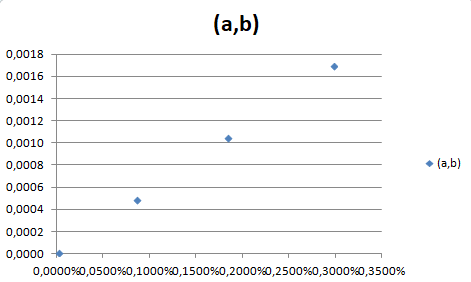
\includegraphics[scale=1]{same_ratio_ab}
\caption{(a,b) pairs ordered by increasing tenor}
\label{fig:same_ratio_ab}
\end{figure}

Therefore, differences between incremental and not incremental calibration are reduced to liquidity choice in order to perform a better global calibration, because the analysis which follows are exactly the same.

\subsection{Relative basis maximum value as difference of the absolute ones}

Furthermore, fixing $c$ and $t_{max}$ between relative and absolute basis means posing a bound on the relative basis maximum. 

Given:

\begin{equation*}
    s_{x}(t_{max})=\frac{b_{x}}{c} e^{(\frac{a_{x}c}{b_{x}}-1)} +d_{x}
\end{equation*}

and

\begin{equation*}
    s_{y}(t_{max})=\frac{b_{y}}{c} e^{(\frac{a_{y}c}{b_{y}}-1)} +d_{y}\,,
\end{equation*}

with:

\begin{equation*}
    \frac{a_{x}}{b_{x}}=\frac{a_{y}}{b_{y}}=\frac{a}{b}\,,
\end{equation*}

it follows that

\begin{equation*}
    s_{x}(t_{max})=\frac{b_{x}}{c} e^{(\frac{a c}{b}-1)} +d_{x}
\end{equation*}

and

\begin{equation*}
    s_{y}(t_{max})=\frac{b_{y}}{c} e^{(\frac{a c}{b}-1)} +d_{y}
\end{equation*}

If $s_{x,y}(t_{max})$ is located in the same point of time, the maximum of the relative basis is:

\begin{equation*}
    s_{x,y}(t_{max})=s_{x}(t_{max})-s_{y}(t_{max})\,.
\end{equation*}

Therefore:

\begin{equation*}
    s_{x,y}(t_{max})=\frac{b_{x}-b_{y}}{c} e^{(\frac{a c}{b}-1)} +(d_{x}-d_{y})\,,
\end{equation*}

\begin{equation*}
    s_{x,y}(t_{max})=\frac{b_{x,y}}{c_{x,y}} e^{(\frac{a_{x,y} c_{x,y}}{b_{x,y}}-1)} +(d_{x,y})\,,
\end{equation*}

which is the relative basis maximum functional form.

\subsection{Dominated d}

Given that from an implementation point of view the validity of an abcd basis depends on the satisfaction of particular run time requirements both on the parameters:

\begin{itemize}
    \item $c>0$, otherwise the basis explodes;
    \item $d>=0$, otherwise the long run value is negative;
    \item $a+d>=0$, otherwise the basis starting point is negative;
\end{itemize}

and on the one and only stationary point:
\begin{itemize}
    \item$b>=-e^{\left(1-\frac{c a}{b}\right)}d c$\,, 
otherwise a negative value at the stationary point can raise, which should be the maximum (and a negative one makes no sense for the basis);
\end{itemize}

the numerical procedure cannot estimate parameters which do not respect the validity constrained, but the basis shifting can lead to the not satisfaction of them, such that the basis is not well-formed.
In order to avoid it, a further step is needed. 

Considering that for "basis shifting" $c_{x,y}$ is taken from the absolute basis calibration and plugged in an exogenous way into the relative basis functional form, while $a_{x,y}$ and $b_{x,y}$ should satisfy a particular relation, the only parameter which may be arbitrary moved in order to well-form the basis is $d_{x,y}$.

Therefore, in the following $d_{x,y}$ is tuned according to the rule "given x and y tenors, where $x>y$, if $d_{x}<d_{y}$ then $d_{x}=d_{y}+\epsilon$" where $\epsilon$ is a negligible quantity. This rule allows to reach the goal with a small impact, indeed as above shown the difference in d for 3M, 6M and 12M is negligible and the impact on the quality of repricing is negligible too.

Considering the parameters of a relative basis $s_{x,y}$, it empirically holds that:

\begin{itemize}
    \item $c_{x}=c_{y}=c_{x,y}>0$, because $c_{x}$ satisfies the same positive constraint;
    \item $d_{x,y}>=0$, by construction;
    \item $a_{x,y}+d_{x,y}>=0$, given a pair of tenors x and y, with $x>y$, $a_{x}>a_{y}$, because of linearity property, and $d_{x,y}>=0$;
    \item $ b_{x,y}>=-e^{\left(1-\frac{c_{x,y} a_{x,y}}{b_{x,y}}\right)}d_{x,y} c_{x,y}$, d times $c$ and the exponential term are always positive, it follows that the equation is always satisfied if $b_{x,y}>=0$, which is guaranteed by the linearity relation between $a_{x}$ and $b_{x}$ .
\end{itemize}

Therefore, with this trick the relative basis is always well-formed with a low impact on the calibration.

The algorithm consists in:

\begin{itemize}
    \item $t_{max}$ and $c$ global calibration;
    \item evaluation of $d$ dominance;
    \item eventual application of the "$d$ trick", which means to internally fix d according to the dominated $d$ rule, exploiting the possibility to fix the parameters, and then re-calibrating the model.
\end{itemize}

Note: it makes sense because empirically if it happens that for a tenor $x$ greater than $y$ $d_{x}<d_{y}$ it is possible to make it an equality equation just adding an $\epsilon$ quantity on the left side: $d_{x}+\epsilon=d_{y}$. Otherwise a $d$ constrained calibration would be required.

\subsection{Empirical results}

Considering both the global error described by \eqref{eq:global_error} which still takes a value of 2.13, confirming the goodness of the $d$ trick, and the correction factor distribution, the results are excellent:

\begin{figure}[H]
\centering
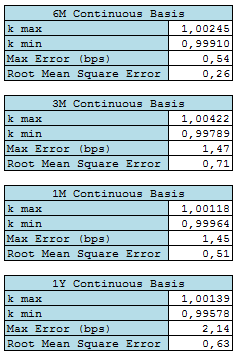
\includegraphics[scale=1]{k_no_inc_t_c_d}
\caption{Correction factors k from not incremental calibration with dominated d, global $t_{max}$ and c}
\label{fig:k_no_inc_t_c_d}
\end{figure}

Range of $k$ values is closed to 1 that is the best value because indicates that no corrections are needed.
Moreover, the statistics follow:

\begin{figure}[H]
\centering
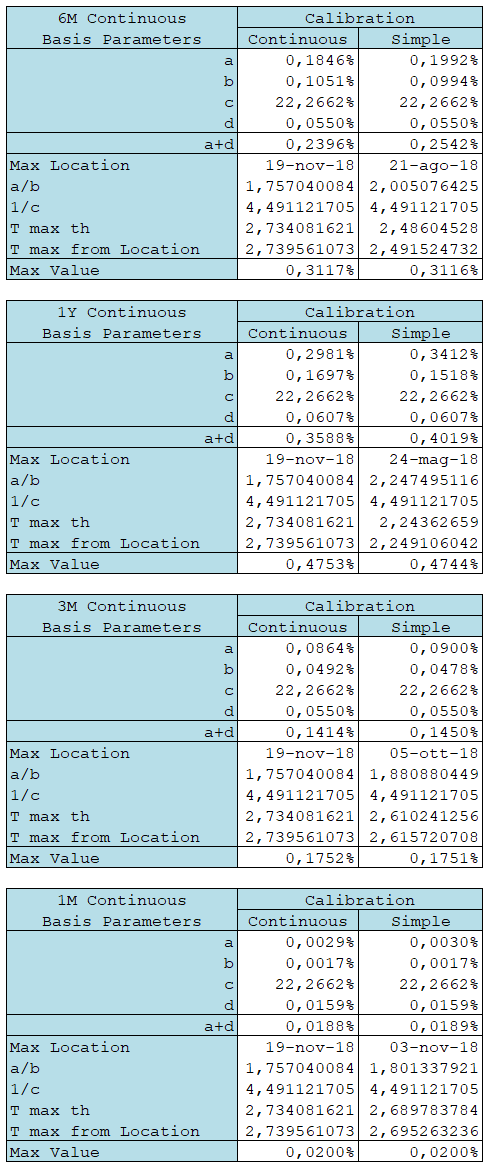
\includegraphics[scale=1]{acdt_Parameters_t_c_d}
\caption{Parameters from not incremental calibration with dominated d, global $t_{max}$ and c}
\label{fig:acdt_Parameters_t_c_d}
\end{figure}

All the previous considerations without the d trick are still comfortably valid meaning that the correction is a "free meal" which allows to get all the advantages without losing model capability to fit the market.

Once again, although remembering that the index which points to an acdt basis should be corrected with the k factors in order to perfectly reprice the provided market quotes, it is interesting to look at the repricing errors for each tenor:

\begin{figure}[H]
\centering
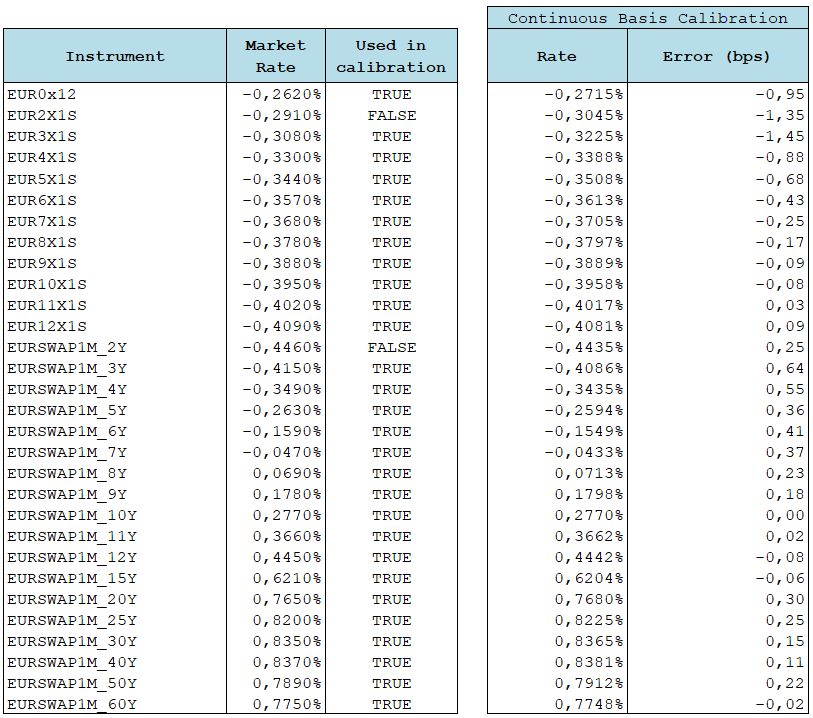
\includegraphics[scale=1]{1Merror_t_c_d}
\caption{1M instruments index repricing errors with dominated d, global $t_{max}$ and c}
\label{fig:1Merror_t_c_d}
\end{figure}

\begin{figure}[H]
\centering
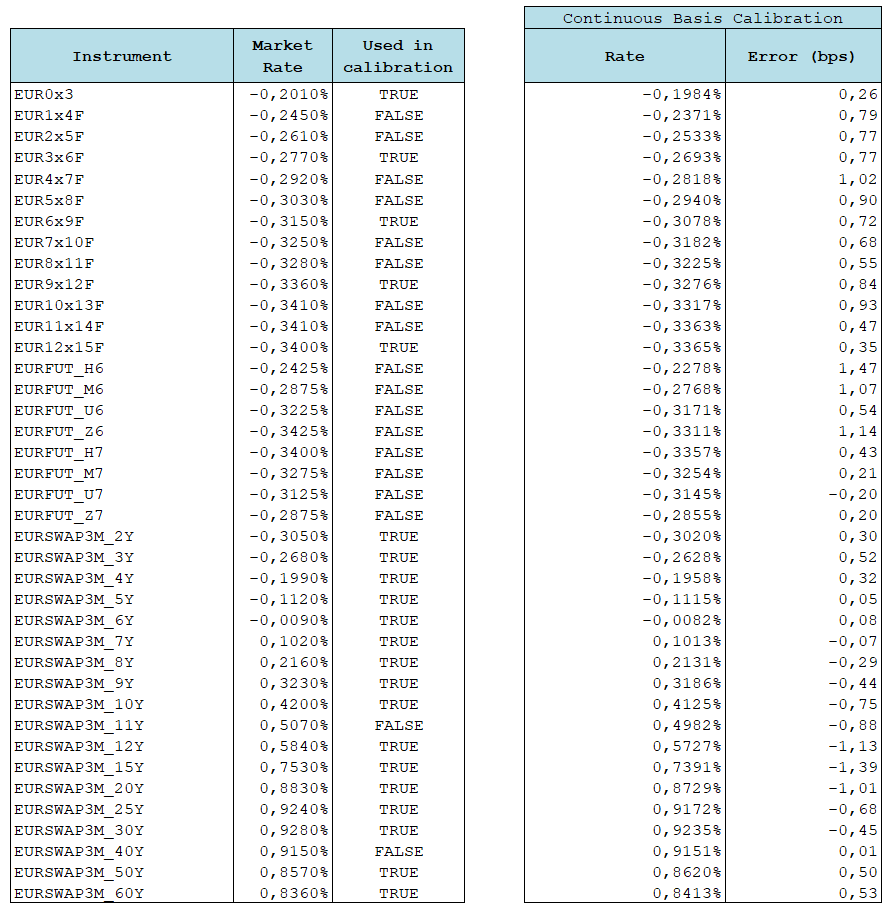
\includegraphics[scale=1]{3Merror_t_c_d}
\caption{3M instruments index repricing errors with dominated d, global $t_{max}$ and c}
\label{fig:3Merror_t_c_d}
\end{figure}

\begin{figure}[H]
\centering
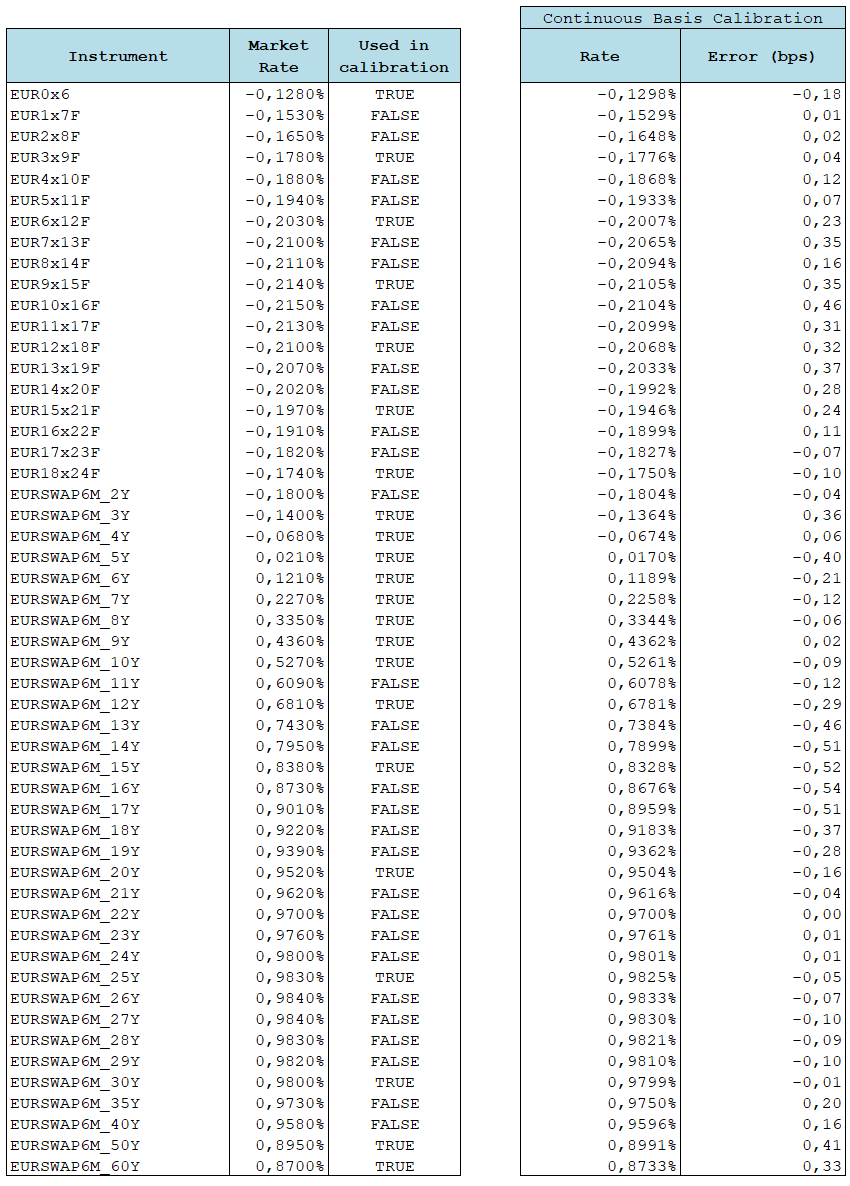
\includegraphics[scale=1]{6Merror_t_c_d}
\caption{6M instruments index repricing errors with dominated d, global $t_{max}$ and c}
\label{fig:6Merror_t_c_d}
\end{figure}

\begin{figure}[H]
\centering
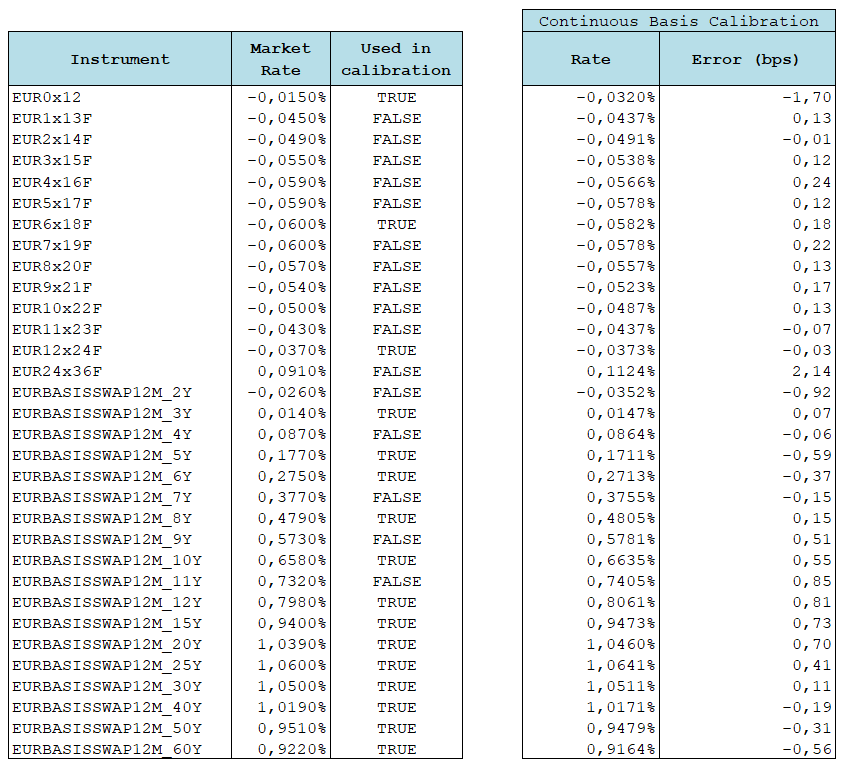
\includegraphics[scale=1]{12Merror_t_c_d}
\caption{12M instruments index repricing errors with dominated d, global $t_{max}$ and c}
\label{fig:12Merror_t_c_d}
\end{figure}

The main findings from this empirical evaluation are:

\begin{itemize}
    \item goodness of fitting which demonstrates the validity of the approach;
    \item possibility to shift to incremental basis.
\end{itemize}

\subsection{Basis shifting empirical results}

The empirical research is concluded investigating the k values, looking at the parameters and the repricing errors for the shifted relative basis.

As it is possible to observe, the statistics are the same of the ones for the relative basis as expected, it happens because of the structure which arises imposing the constraints on $t_{max}$ and $c$:

\begin{figure}[H]
\centering
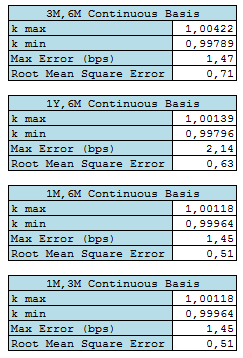
\includegraphics[scale=1]{k_no_inc_t_c_d_rel}
\caption{Relative basis correction factors k from not incremental calibration with dominated d, global $t_{max}$ and c}
\label{fig:k_no_inc_t_c_d_rel}
\end{figure}

\begin{figure}[H]
\centering
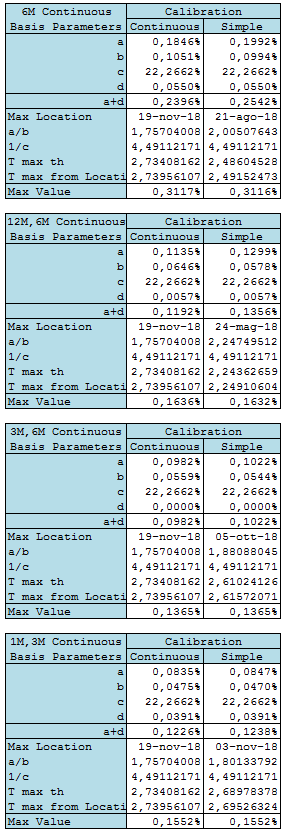
\includegraphics[scale=1]{acdt_Parameters_t_c_d_rel}
\caption{Relative Basis parameters from not incremental calibration with dominated d, global $t_{max}$ and c}
\label{fig:acdt_Parameters_t_c_d_rel}
\end{figure}

Just for reporting an example:

\begin{figure}[H]
\centering
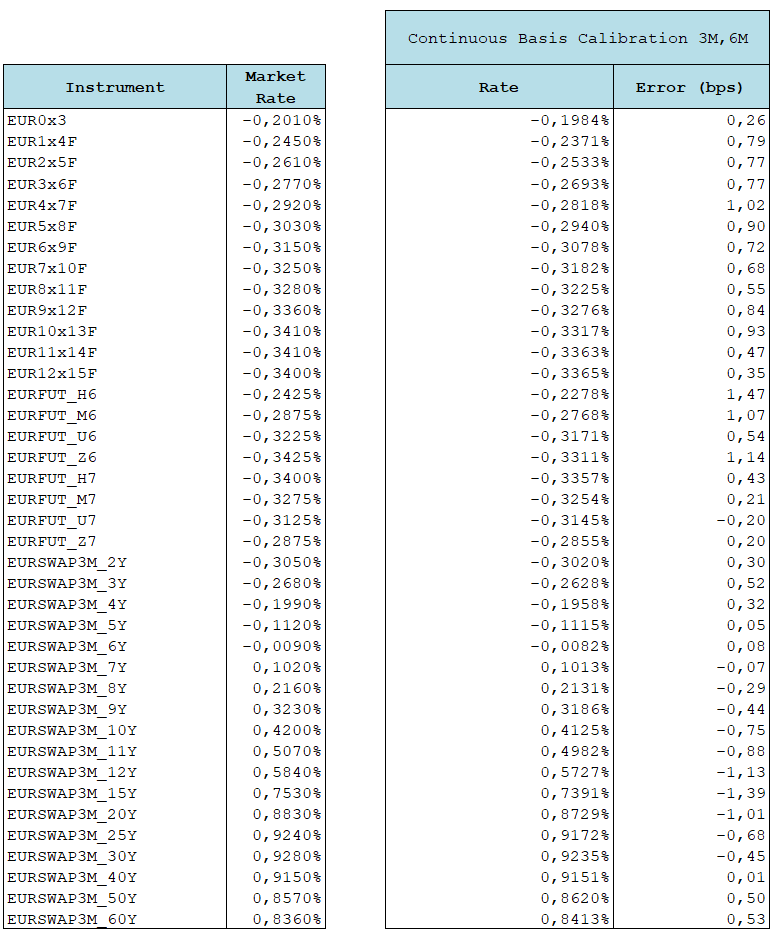
\includegraphics[scale=1]{3M6Merror_t_c_d}
\caption{1M instruments relative basis 4M,6M index repricing errors with dominated d, global $t_{max}$ and c}
\label{fig:3M6Merror_t_c_d}
\end{figure}

Moreover, also the repricing error for $s_{1M,6M}$ and $s_{1M,3M}$ are the same, because the indifference between:

\begin{equation*}
    f_{1M}=f_{ON} + s_{6M} - s_{1M,6M}
\end{equation*}

and

\begin{equation*}
    f_{1M}=f_{ON} + s_{3M} - s_{1M,3M}\,,
\end{equation*}

more generally is valid that:

\begin{equation*}
    f_{x}=f_{ON} + s_{y} \mp s_{x,y}  \forall y\,,
\end{equation*}

because of the additive property of the basis.

Indeed, given 3 generic tenors $x$, $y$ and $z$, it always true that:

\begin{equation*}
   s_{x}= s_{y} \mp s_{x,y} 
\end{equation*}

and 

\begin{equation*}
   s_{x}= s_{z} \mp s_{x,z} \,.
\end{equation*}

Continuing the empirical validation of theoretical results, the basis time of maximum coincides although not explicitly forced to be on the same point of time.
Considering both the $a$ values for the absolute basis together with the ones for the relative, it is empirically verified the linearity property above enunciated:

\begin{figure}[H]
\centering
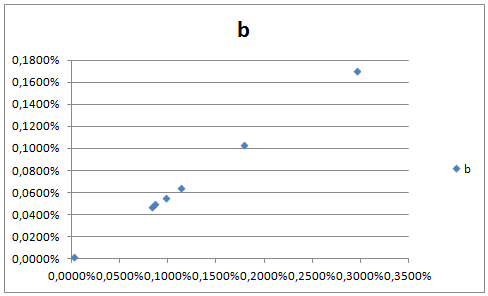
\includegraphics[scale=1]{same_ratio_a_b_rel}
\caption{(a,b) pairs ordered by increasing tenor from relative and absolute basis}
\label{fig:same_ratio_a_b_rel}
\end{figure}

ordering the tenor basis according to the following table is possible to evaluate it numerically:

\begin{figure}[H]
\centering
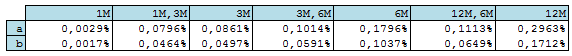
\includegraphics[scale=0.8]{tenorbasis_linearity_prop}
\caption{(a,b) pairs ordered by increasing tenor, relative and absolute basis}
\label{fig:tenorbasis_linearity_prop}
\end{figure}

discovering that 0.58 is the value for $x$ such that: $b=a*x$.


The relations about $s_{x,y}(t_{max})$ and $s_{x}(t_{max})$ are verified. It is possible to appreciate the presence of a structure not only on the common value of $t_{max}$ for each basis, but also an additive one on $s_{x,y}(t_{max})$ which has been spotted as a meaningful parameter at the beginning of the thesis:

\begin{figure}[H]
\centering
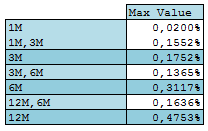
\includegraphics[scale=1]{max_value_structure}
\caption{Tenor Basis maximum structure}
\label{fig:max_value_structure}
\end{figure}




Concluding, the absolute basis 

\begin{figure}[H]
\centering
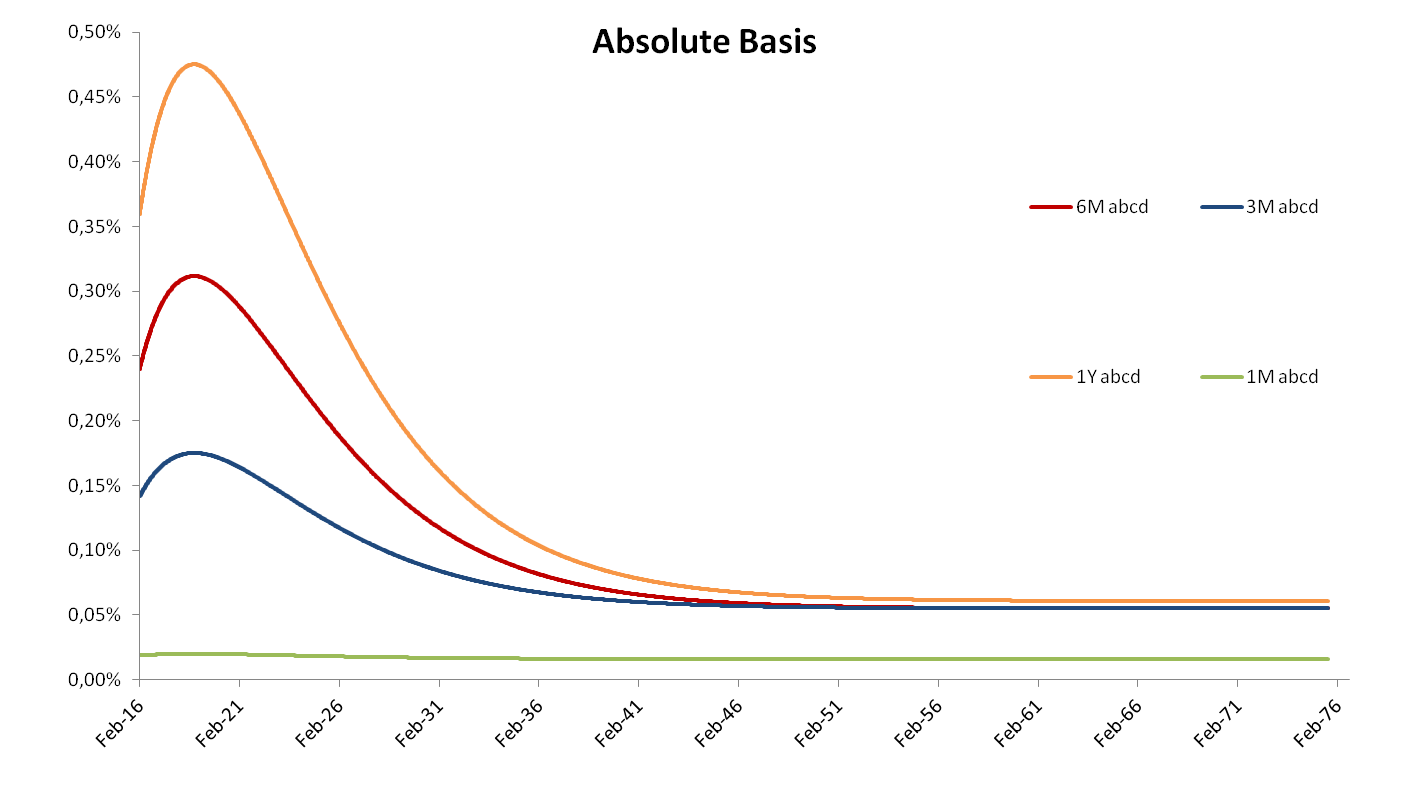
\includegraphics[scale=0.55]{graph_absolute_basis_comparison_no_inc_t_c_d}
\caption{Absolute Basis comparison}
\label{fig:graph_basis_comparison_no_inc_t_c_d}
\end{figure}

and the relative one:

\begin{figure}[H]
\centering
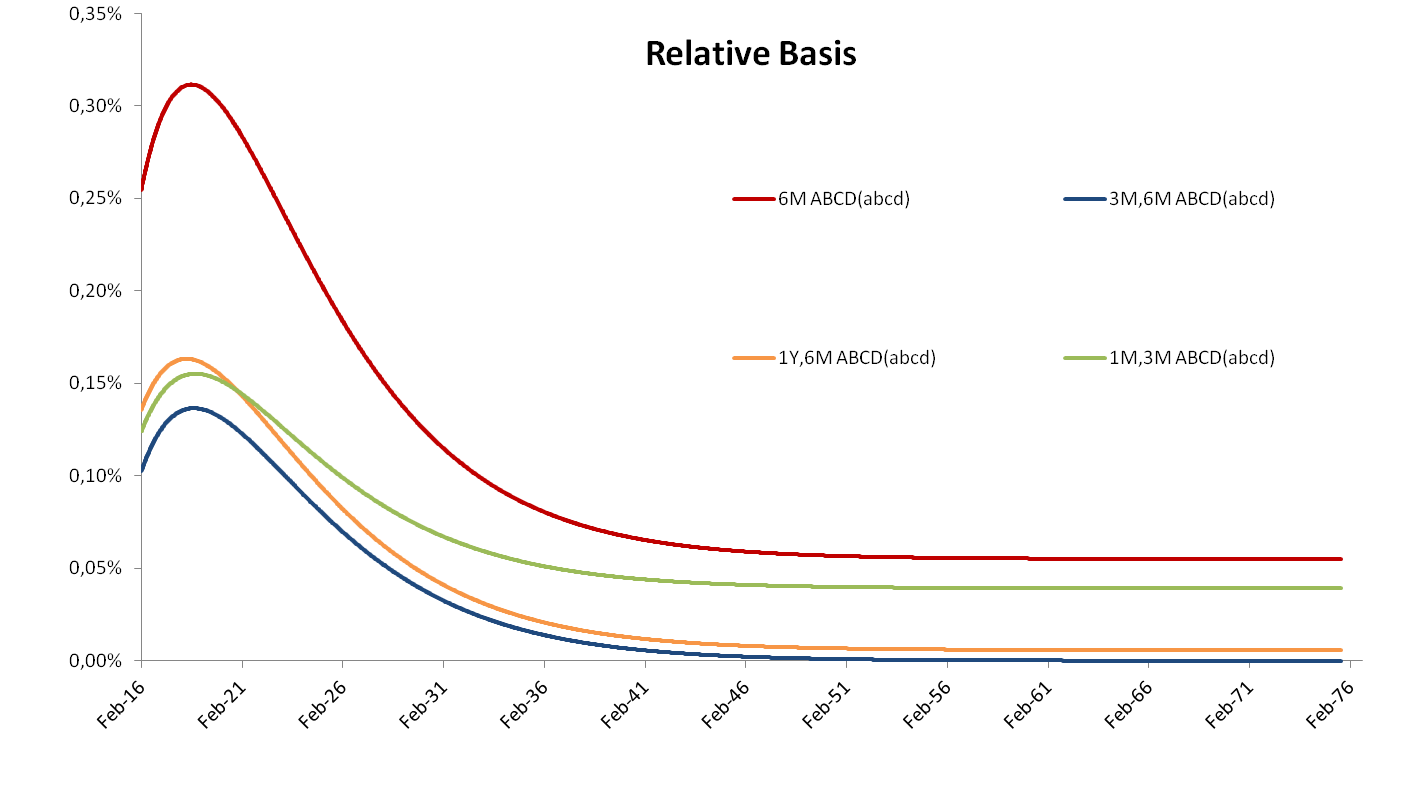
\includegraphics[scale=0.55]{graph_relative_basis_comparison_no_inc_t_c_d}
\caption{Relative Basis comparison}
\label{fig:graph_relative_basis_comparison_no_inc_t_c_d}
\end{figure}

show all the above mentioned features.
